
\section{The PETALO concept}
\label{sec.petalo}

The first idea of using a Liquid Xenon Time Projection Chamber (LXeTPC) for PET was proposed in 1993 by Chepel \cite{chepel02}. The proposed detector was a LXe multi-wire detector consisting of six ionization cells, each formed by two parallel cathode plates with a multi-wire anode in the middle. 
Subsequent R\&D is documented in \cite{chepel94,chepel95,lopes95,chepel97,crespo98,chepel99,crespo00}. {\bf All those devices were based in the exploration of the ionization signal in LXe}. {\em However, the measurement of such signals introduces a severe constrain to the technique, given the slow drift time of electrons in LXe} (typically of the order of 2 mm/$\mu$s, for a drifting field of 1 KV/cm). Since $\lambda = 3$.6~cm the practical length of a LXe cell (along the photon line of flight) must be of 5 cm to contain 77 \% of the photons. This, in turn, implies drifting times of 25 $\mu$s, which limits the interaction rate that can be recorded by the cell to $\sim10^5 s^{-1}$, and therefore imposes a low-rate PET with a limited range of applications. 

On the other hand, the possibility of building a LXe PET (with TOF capabilities) based on the excellent properties of LXe as scintillator, was first suggested by Lavoie in 1976 \cite{lavoie76} , and the study of this type of PET was carried out by the Waseda group \cite{doke06,nishikido05,nishikido04}. The Waseda prototype (see Figure \ref{fig.waseda}) was based in LXe cells read out by VUV-sensitive PMTs. In those cells one of the sides was left instrumented. The relatively poor performance of the system can be attributed in part to the use of PMTs and in part to the partial lack of instrumentation which affected both the energy and the time resolution. The PMTs, although sensitive to the VUV light emitted by xenon had low quantum efficiencies (in the range 5-25 \%), and their rather large size compared with the size of the cell ($18\times 18$~mm$^2$) introduced significant geometrical effects which were difficult to correct. As a result of the above effects combined the energy resolution was of the same order than that of conventional SSDs. The space resolution was rather good, in the range of 2-3 mm, but only in the central volume of the cell (a cube of 5 mm size), and deteriorated rapidly in the borders, due to the space corrections introduced by the (relatively) large PMTs. The time resolution in the central volume was excellent, of the order of 260 ps, showing the enormous potential of the technology for PET application.

\begin{figure}[!htb]
	\begin{center}
           \subfloat[]{
               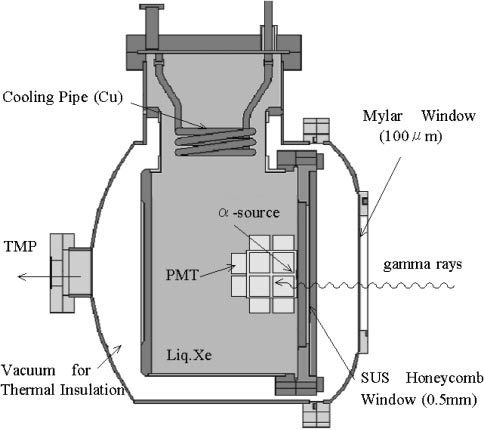
\includegraphics[width=.5\textwidth]{img/waseda1.png}
           }
           \subfloat[]{
               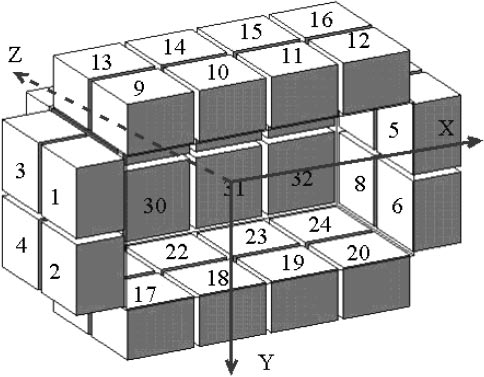
\includegraphics[width=.5\textwidth]{img/waseda2.png}
           }
           \caption{\label{fig.waseda} Illustration of Waseda's group prototype taken from \cite{nishikido05}. (a) Cross-sectional view of the prototype liquid Xe PET detector. (b) Arrangement of 32 PMTs.}
    \end{center}
\end{figure}

PETALO (Positron Emission TOF Apparatus base on Liquid xenOn) is a new concept for a TOF-capable, high sensitivity, PET apparatus based in the excellent scintillating properties of LXe and the concept of a new type of detection cell, which captures with high efficiency, minimal border effects and uniform response, most of the light produced.
 
\begin{itemize} 
\item {\bf High efficiency} is achieved by covering the internal side of the cell with reflective panels, made of high density teflon coated with TPB. The emitted ultraviolet light (172 nm) is shifted to 420 nm as soon as it hits the teflon panels, which on the other hand, reflect blue light in the range of 420 nm with 98-99\% efficiency. Furthermore, TPB does not absorb blue light above 400 nm, therefore minimising loses. 
\item {\bf High homogeneity and uniform response}, with minimal border effects is achieved by choosing SiPMs as readout devices. Currently, several manufacturers offer SiPMs of large area, high gain, low dark current and very low noise which can operate at liquid xenon temperatures with excellent performance.  
\item {\bf Excellent energy resolution} is achieved thanks to the hight light yield of LXe and the homogeneity of the cell (the measured energy varies very little from one point of the cell to the other).  
\item {\bf Good spatial resolution in the three coordinates} is possible by using the SiPMs array covering the entry and exit face of the cell with SiPMs which provide the transverse (x-y) coordinates and using the ratio of light recorded in the entry and exit face to measure the longitudinal (z) coordinate. 
\item {\bf Excellent CRT} is possible thanks to the fast decay scintillation time of LXe (2.2 ns) and the fast response of the SiPMs.  
\end{itemize} 
